\documentclass[11pt]{article}
\usepackage[margin=1in]{geometry} 
\usepackage{titlesec}
\usepackage{amsmath,amsthm,amssymb,amsfonts}
\usepackage{graphicx,epstopdf,fancyhdr,xspace,algorithm,algorithmic}
\usepackage[space]{grffile}
\pagestyle{fancy}
\usepackage{epsfig}
\usepackage[space]{grffile}
\usepackage{titlesec}
\usepackage[table]{xcolor}
\usepackage[hyphens]{url}
\usepackage{enumitem} % package used to generate bulleted lists 
\usepackage{tikz}
\usetikzlibrary{arrows,automata}
\theoremstyle{definition}
\renewcommand{\epsilon}{\varepsilon}
\newtheorem{problem}{Problem} %
\cfoot{\thepage}
\renewcommand{\headrulewidth}{0.4pt}
\renewcommand{\headwidth}{\textwidth}
\renewcommand{\footrulewidth}{0.4pt}


\newcommand{\mymin}{\ensuremath{\mbox{\sc FindMin}}\xspace} 
\newcommand{\ms}{\ensuremath{\mbox{\sc Mergesort}}\xspace} 
\newcommand{\qs}{\ensuremath{\mbox{\sc Quicksort}}\xspace} 

\newtheorem{claim}{Claim}
\newtheorem{definition}{Definition}
\newtheorem{theorem}{Theorem}
\newtheorem{lemma}{Lemma}
\newtheorem{observation}{Observation}
\newtheorem{question}{Problem}
\titleformat*{\section}{\large\bfseries}
\newcommand{\N}{\mathbb N} %you can define shorthands this way, here we are defined \N as a shorthand for math bold N for natural numbers
\newenvironment{solution}{\bigskip\noindent{\it Solution.}  \ignorespaces}{\hfill\qed}
\usepackage{hyperref}
\usepackage{hyperref}
\hypersetup{
    colorlinks=true,
    linkcolor=blue,
    filecolor=magenta,      
    urlcolor=cyan,
}
\urlstyle{same}
\PassOptionsToPackage{hyphens}{url}
\newcommand{\homework}[6]{
   \pagestyle{myheadings}
   \thispagestyle{plain}
   \newpage
   \setcounter{page}{1}
   \noindent
   \begin{center}
   \framebox{
      \vbox{\vspace{2mm}
    \hbox to 6.28in { {\bf CS256:~Algorithm Design and Analysis \hfill #1} }
       \vspace{6mm}
       \hbox to 6.28in { {\Large \hfill #2 \normalsize{(#3)}  \hfill} }
       \vspace{6mm}
     \hbox to 6.28in { {\it Instructor: #4 \hfill  Solution template: #5} }
   }
   }
   \end{center}
   \markboth{#1}{#1}
   \vspace*{4mm}
}

\begin{document}
\homework{Spring 2021}{Assignment 3}{due 03/17/2021 }{Shikha Singh}{\href{https://www.overleaf.com/read/wbvwffqgqpsw}{\em Overleaf}}

\subsection*{Greedy and Exchange Argument}
\begin{question}
At your summer job, you are made in charge of storing books on shelves in a library.  Consider $n$ books where each book $i$ has some thickness $t_i$.
The order of storing the books is fixed by the cataloging system and so you cannot rearrange them. 
 Every shelf in the library has a fixed length $L$.  Suppose any book fits on
any shelf by itself. Design an algorithm to store all the $n$ books using the fewest number of shelves possible. Show that your algorithm is correct.
\end{question}

\begin{solution}
\end{solution}


\newpage

\begin{question} 
Let $X$ be a set of $n$ intervals on the real line. We say that a set $P$ of points
stabs $X$ (or is \emph{the stabbing set}) if every interval in $X$ contains at least one point in $P$. See Figure~\ref{fig:stabbing}. In this and the next question, we will design and analyze an efficient algorithm to compute minimum set of points that
stabs $X$. Assume that your input consists of pairs ($\ell_i$, $r_i$), representing the left and right endpoints of $i$th interval in $X$, for $1\leq i \leq n$. 

\begin{figure}[h]\label{fig:stabbing}
\centering
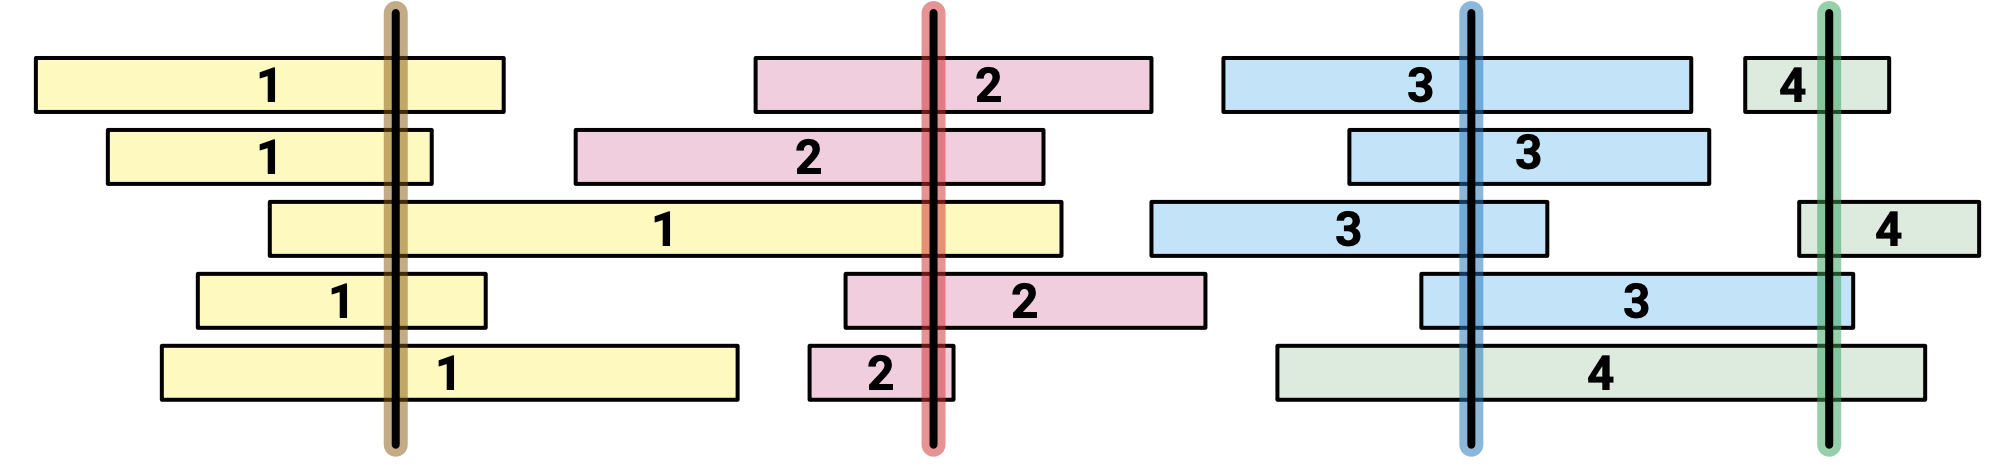
\includegraphics[scale=0.15]{stabbing.png}\caption{A set of intervals stabbed by four points. From Jeff Erickson's \href{www.algorithms.wtf}{Algorithms book}.}
\end{figure}
\vspace{-10pt}



\begin{enumerate}[noitemsep, label = (\alph*), leftmargin=*]
 
    \item\label{parta} \emph{Structure of optimal.} If we were to choose stabbing points anywhere on the intervals, the possibilities would be endless.  So first, we prove a structural property about any optimal solution to the problem, as this will guide our algorithm design.  Show that for any set of intervals, there exists an optimal solution (a stabbing set of minimum size) where every stabbing point is the right endpoint $r_i$ of some interval. This means that without loss of generality (WLOG), we can restrict ourselves to stabbing sets that satisfy this property. 


\begin{solution}
\end{solution}


   
\item  Consider the following greedy strategy: sort the intervals in increasing order of their right endpoints. Take the first interval from this list, and add its right endpoint to the stabbing set. Remove all intervals that contain this point. Repeat until no intervals remain. Clearly, this produces a valid stabbing set, but is it optimal? 

Prove that the above greedy strategy is optimal, that is, it produces a stabbing set of minimum size. (Use part~\ref{parta} and an exchange argument.)
 
\begin{solution}
\end{solution}



\item Analyze the running time of the greedy strategy and show that it can be implemented in $O(n \log n)$ time.

\begin{solution}
\end{solution}


     
\end{enumerate} 
\end{question}

\newpage

\subsection*{Greedy Algorithms on Graphs}


\begin{question} Are the following statements True of False?  You must justify your choice with a brief explanation or a counterexample.


\begin{enumerate} [label = (\alph*), leftmargin = *, noitemsep]

\item The minimum spanning tree of a graph includes the minimum-weight edge in {\em every} cycle.

\begin{solution}
\end{solution}

\item Kruskal’s algorithm for finding minimum spanning trees works for negative edge weights.

\begin{solution}
\end{solution}

\item Dijkstra's shortest path algorithm works even when the graph has negative edge weights.


\begin{solution}
\end{solution}
\end{enumerate}
\end{question}

\newpage

\begin{question} 
It is often the case that updating the output of an algorithm when the input changes is easier than computing it from scratch.
One such example is that of dynamically changing edge weights in a graph.  This problem asks you to consider how you would maintain a minimum-cost spanning tree in
such an environment.  Suppose you are given a graph $G$ with weighted edges and a minimum spanning tree $T$ of $G$. 
		

	Describe and analyze an algorithm to update the minimum spanning tree when the weight of a single edge $e$ is decreased.\footnote{Food for thought: what if we increase the weight of a single edge? What do we update the MST then?}  
	 The input to your algorithms is the edge $e$ and its new weight and your algorithms should modify $T$ so that it is still a minimum spanning tree.  Remember to prove correctness and analyze the running time of your algorithm.
 
Assume that all edge costs are distinct. 
 {\em Hint:  Consider $e \in T$ and $e \not\in T$ separately and use the properties that relate MST, cycles, and cuts.}
\end{question}


\begin{solution}
\end{solution}

\newpage


\begin{question} \label{q:fes}
A {\em feedback edge set} in a graph $G$ is a subset $F$ of the edges of $G$ such that every cycle in $G$ contains at least one edge in $F$.  In other words, removing every edge in $F$ makes the graph $G$ acyclic.  
Notice that the set of all the edges of the graph trivially forms a feedback edge set.    

\begin{enumerate} [label = (\alph*), leftmargin = *, noitemsep]
\item\label{item:a} Let a feedback edge set $F$ be {\em minimal} if it does not have another feedback edge set as its subset, that is, 
there is no set $F' \subset F$ such that $F'$ is also a feedback edge set.\footnote{Note that this has nothing to do with edge costs!} 
Show that if $T$ is a spanning tree of $G$, then $F = E -T$ is a minimal feedback edge set.


\begin{solution}  
\end{solution}



\item\label{item:b} Show that if $F$ is a minimal feedback edge set of $G$, then the edges $E - F$ form a spanning tree $T$ of $G$. 

	\begin{solution}  
\end{solution}


\item Use parts~\ref{item:a} and~\ref{item:b} to give an algorithm to compute the {\em minimum-weight} feedback-edge set of a given edge-weighted graph.
Argue the correctness and runtime of your algorithm.
(Assume that $G$ is connected and all its edge weights
are distinct and positive.)

\begin{solution}  
\end{solution}


\end{enumerate}
\end{question}




\newpage
\subsection*{Acknowledgment}
This is where you cite your sources and collaborators.


\end{document}



